\documentclass{standalone}
\usepackage{tikz}
\usetikzlibrary{patterns, positioning}


\begin{document}
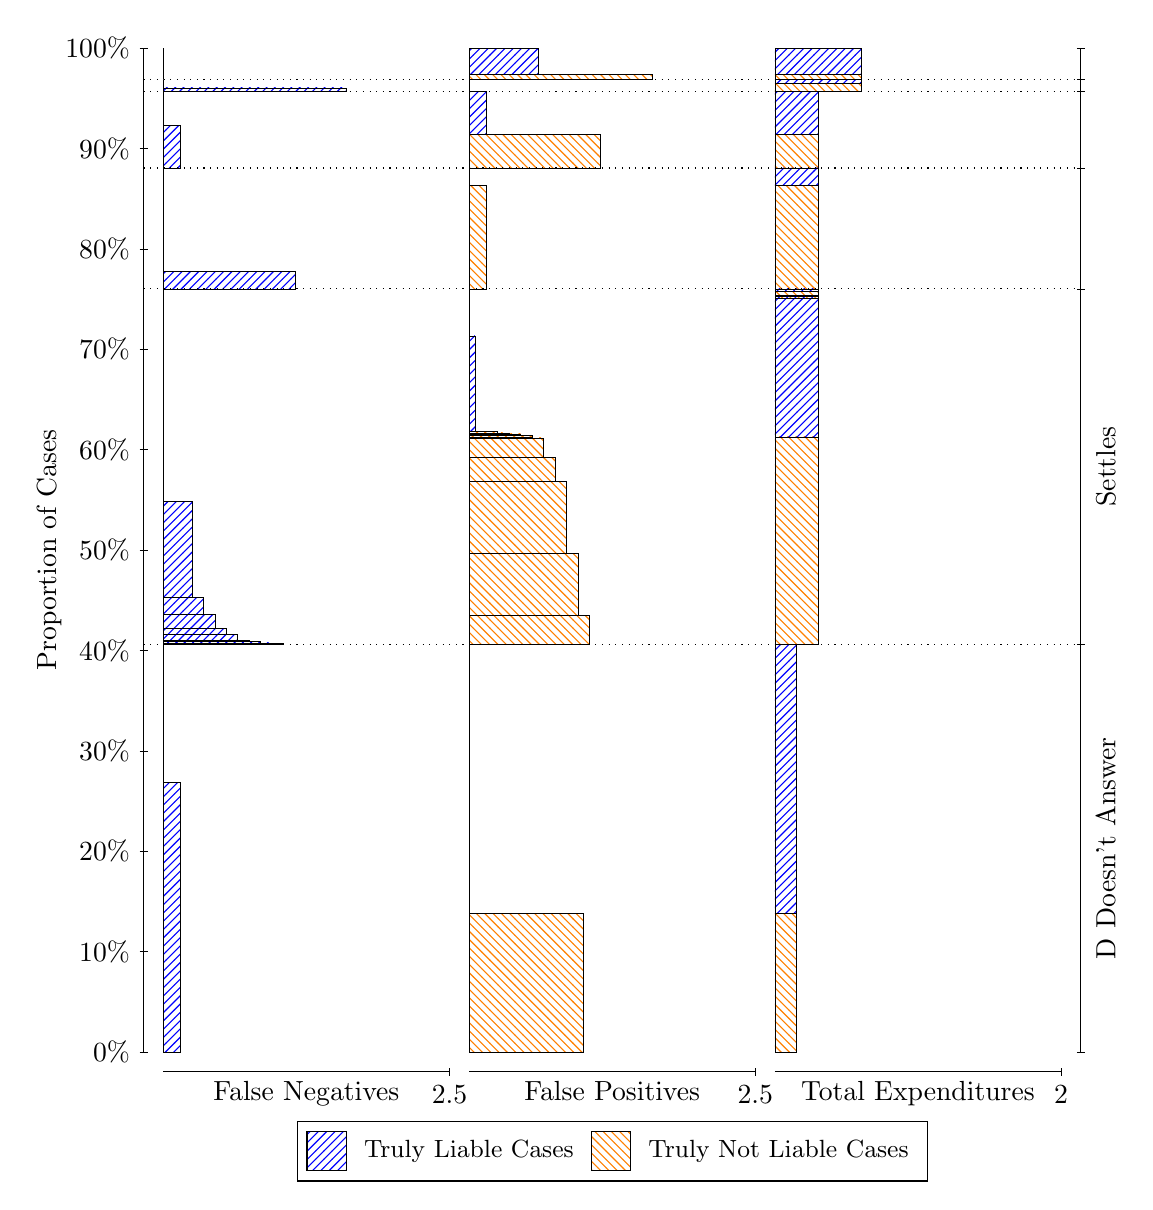
\begin{tikzpicture}
\draw[black, very thin] (1.5,1.75) -- (1.5,14.5);
\node[rotate=90, text=black, anchor=center] at (0.3, 8.125) {Proportion of Cases};
\draw[black, very thin] (1.45,1.75) -- (1.55,1.75);
\node[text=black, anchor=east] at (1.45, 1.75) {0\%};
\draw[black, very thin] (1.45,3.025) -- (1.55,3.025);
\node[text=black, anchor=east] at (1.45, 3.025) {10\%};
\draw[black, very thin] (1.45,4.3) -- (1.55,4.3);
\node[text=black, anchor=east] at (1.45, 4.3) {20\%};
\draw[black, very thin] (1.45,5.575) -- (1.55,5.575);
\node[text=black, anchor=east] at (1.45, 5.575) {30\%};
\draw[black, very thin] (1.45,6.85) -- (1.55,6.85);
\node[text=black, anchor=east] at (1.45, 6.85) {40\%};
\draw[black, very thin] (1.45,8.125) -- (1.55,8.125);
\node[text=black, anchor=east] at (1.45, 8.125) {50\%};
\draw[black, very thin] (1.45,9.4) -- (1.55,9.4);
\node[text=black, anchor=east] at (1.45, 9.4) {60\%};
\draw[black, very thin] (1.45,10.675) -- (1.55,10.675);
\node[text=black, anchor=east] at (1.45, 10.675) {70\%};
\draw[black, very thin] (1.45,11.95) -- (1.55,11.95);
\node[text=black, anchor=east] at (1.45, 11.95) {80\%};
\draw[black, very thin] (1.45,13.225) -- (1.55,13.225);
\node[text=black, anchor=east] at (1.45, 13.225) {90\%};
\draw[black, very thin] (1.45,14.5) -- (1.55,14.5);
\node[text=black, anchor=east] at (1.45, 14.5) {100\%};

\draw[black, very thin] (13.4,1.75) -- (13.4,14.5);
\draw[black, very thin] (13.35,1.75) -- (13.45,1.75);
\node[anchor=west] at (13.35, 1.75) {};
\draw[black, very thin] (13.35,6.928) -- (13.45,6.928);
\node[anchor=west] at (13.35, 6.928) {};
\draw[black, very thin] (13.35,11.441) -- (13.45,11.441);
\node[anchor=west] at (13.35, 11.441) {};
\draw[black, very thin] (13.35,12.977) -- (13.45,12.977);
\node[anchor=west] at (13.35, 12.977) {};
\draw[black, very thin] (13.35,13.947) -- (13.45,13.947);
\node[anchor=west] at (13.35, 13.947) {};
\draw[black, very thin] (13.35,14.101) -- (13.45,14.101);
\node[anchor=west] at (13.35, 14.101) {};
\draw[black, very thin] (13.35,14.5) -- (13.45,14.5);
\node[anchor=west] at (13.35, 14.5) {};

\draw[black, very thin, pattern color=blue, pattern=north east lines] (1.75,1.75) rectangle (1.968,5.1719);
\draw[black, very thin, pattern color=orange, pattern=north west lines] (1.75,5.1719) rectangle (1.75,6.928);
\draw[black, very thin, pattern color=blue, pattern=north east lines] (1.75,6.928) rectangle (3.276,6.9388);
\draw[black, very thin, pattern color=blue, pattern=north east lines] (1.75,6.9388) rectangle (3.1307,6.9462);
\draw[black, very thin, pattern color=blue, pattern=north east lines] (1.75,6.9462) rectangle (2.9853,6.9607);
\draw[black, very thin, pattern color=blue, pattern=north east lines] (1.75,6.9607) rectangle (2.84,6.9793);
\draw[black, very thin, pattern color=blue, pattern=north east lines] (1.75,6.9793) rectangle (2.6947,7.0512);
\draw[black, very thin, pattern color=blue, pattern=north east lines] (1.75,7.0512) rectangle (2.5493,7.1261);
\draw[black, very thin, pattern color=blue, pattern=north east lines] (1.75,7.1261) rectangle (2.404,7.3054);
\draw[black, very thin, pattern color=blue, pattern=north east lines] (1.75,7.3054) rectangle (2.2587,7.5255);
\draw[black, very thin, pattern color=blue, pattern=north east lines] (1.75,7.5255) rectangle (2.1133,8.7389);
\draw[black, very thin, pattern color=orange, pattern=north west lines] (1.75,8.7389) rectangle (1.75,11.441);
\draw[black, very thin, pattern color=blue, pattern=north east lines] (1.75,11.441) rectangle (3.4213,11.663);
\draw[black, very thin, pattern color=orange, pattern=north west lines] (1.75,11.663) rectangle (1.75,12.977);
\draw[black, very thin, pattern color=blue, pattern=north east lines] (1.75,12.977) rectangle (1.968,13.521);
\draw[black, very thin, pattern color=orange, pattern=north west lines] (1.75,13.521) rectangle (1.75,13.947);
\draw[black, very thin, pattern color=blue, pattern=north east lines] (1.75,13.947) rectangle (4.0753,13.994);
\draw[black, very thin, pattern color=orange, pattern=north west lines] (1.75,13.994) rectangle (1.75,14.101);
\draw[black, very thin, pattern color=orange, pattern=north west lines] (1.75,14.101) rectangle (1.75,14.17);
\draw[black, very thin, pattern color=blue, pattern=north east lines] (1.75,14.17) rectangle (1.75,14.5);
\draw[black, very thin, pattern color=orange, pattern=north west lines] (5.6333,1.75) rectangle (7.0867,3.5061);
\draw[black, very thin, pattern color=blue, pattern=north east lines] (5.6333,3.5061) rectangle (5.6333,6.928);
\draw[black, very thin, pattern color=orange, pattern=north west lines] (5.6333,6.928) rectangle (7.1593,7.2944);
\draw[black, very thin, pattern color=orange, pattern=north west lines] (5.6333,7.2944) rectangle (7.014,8.0832);
\draw[black, very thin, pattern color=orange, pattern=north west lines] (5.6333,8.0832) rectangle (6.8687,8.997);
\draw[black, very thin, pattern color=orange, pattern=north west lines] (5.6333,8.997) rectangle (6.7233,9.3008);
\draw[black, very thin, pattern color=orange, pattern=north west lines] (5.6333,9.3008) rectangle (6.578,9.5499);
\draw[black, very thin, pattern color=orange, pattern=north west lines] (5.6333,9.5499) rectangle (6.4327,9.5608);
\draw[black, very thin, pattern color=orange, pattern=north west lines] (5.6333,9.5608) rectangle (6.4327,9.5776);
\draw[black, very thin, pattern color=orange, pattern=north west lines] (5.6333,9.5776) rectangle (6.2873,9.6004);
\draw[black, very thin, pattern color=orange, pattern=north west lines] (5.6333,9.6004) rectangle (6.142,9.6122);
\draw[black, very thin, pattern color=orange, pattern=north west lines] (5.6333,9.6122) rectangle (5.9967,9.6298);
\draw[black, very thin, pattern color=blue, pattern=north east lines] (5.6333,9.6298) rectangle (5.706,10.843);
\draw[black, very thin, pattern color=blue, pattern=north east lines] (5.6333,10.843) rectangle (5.6333,11.441);
\draw[black, very thin, pattern color=orange, pattern=north west lines] (5.6333,11.441) rectangle (5.8513,12.755);
\draw[black, very thin, pattern color=blue, pattern=north east lines] (5.6333,12.755) rectangle (5.6333,12.977);
\draw[black, very thin, pattern color=orange, pattern=north west lines] (5.6333,12.977) rectangle (7.3047,13.403);
\draw[black, very thin, pattern color=blue, pattern=north east lines] (5.6333,13.403) rectangle (5.8513,13.947);
\draw[black, very thin, pattern color=orange, pattern=north west lines] (5.6333,13.947) rectangle (5.6333,14.055);
\draw[black, very thin, pattern color=blue, pattern=north east lines] (5.6333,14.055) rectangle (5.6333,14.101);
\draw[black, very thin, pattern color=orange, pattern=north west lines] (5.6333,14.101) rectangle (7.9587,14.17);
\draw[black, very thin, pattern color=blue, pattern=north east lines] (5.6333,14.17) rectangle (6.5053,14.5);
\draw[black, very thin, pattern color=orange, pattern=north west lines] (9.5167,1.75) rectangle (9.7892,3.5061);
\draw[black, very thin, pattern color=blue, pattern=north east lines] (9.5167,3.5061) rectangle (9.7892,6.928);
\draw[black, very thin, pattern color=orange, pattern=north west lines] (9.5167,6.928) rectangle (10.062,9.5608);
\draw[black, very thin, pattern color=blue, pattern=north east lines] (9.5167,9.5608) rectangle (10.062,11.327);
\draw[black, very thin, pattern color=orange, pattern=north west lines] (9.5167,11.327) rectangle (10.062,11.345);
\draw[black, very thin, pattern color=blue, pattern=north east lines] (9.5167,11.345) rectangle (10.062,11.356);
\draw[black, very thin, pattern color=orange, pattern=north west lines] (9.5167,11.356) rectangle (10.062,11.407);
\draw[black, very thin, pattern color=blue, pattern=north east lines] (9.5167,11.407) rectangle (10.062,11.441);
\draw[black, very thin, pattern color=orange, pattern=north west lines] (9.5167,11.441) rectangle (10.062,12.755);
\draw[black, very thin, pattern color=blue, pattern=north east lines] (9.5167,12.755) rectangle (10.062,12.977);
\draw[black, very thin, pattern color=orange, pattern=north west lines] (9.5167,12.977) rectangle (10.062,13.403);
\draw[black, very thin, pattern color=blue, pattern=north east lines] (9.5167,13.403) rectangle (10.062,13.947);
\draw[black, very thin, pattern color=orange, pattern=north west lines] (9.5167,13.947) rectangle (10.607,14.055);
\draw[black, very thin, pattern color=blue, pattern=north east lines] (9.5167,14.055) rectangle (10.607,14.101);
\draw[black, very thin, pattern color=orange, pattern=north west lines] (9.5167,14.101) rectangle (10.607,14.17);
\draw[black, very thin, pattern color=blue, pattern=north east lines] (9.5167,14.17) rectangle (10.607,14.5);
\draw[black, dotted] (1.5,6.928) -- (13.4,6.928);
\draw[black, dotted] (1.5,11.441) -- (13.4,11.441);
\draw[black, dotted] (1.5,12.977) -- (13.4,12.977);
\draw[black, dotted] (1.5,13.947) -- (13.4,13.947);
\draw[black, dotted] (1.5,14.101) -- (13.4,14.101);
\draw[black, very thin] (1.75,1.5) -- (5.3833,1.5);
\node[text=black, anchor=north] at (3.5667, 1.5) {False Negatives};
\draw[black, very thin] (5.3833,1.45) -- (5.3833,1.55);
\node[text=black, anchor=north] at (5.3833, 1.45) {2.5};

\draw[black, very thin] (5.6333,1.5) -- (9.2667,1.5);
\node[text=black, anchor=north] at (7.45, 1.5) {False Positives};
\draw[black, very thin] (9.2667,1.45) -- (9.2667,1.55);
\node[text=black, anchor=north] at (9.2667, 1.45) {2.5};

\draw[black, very thin] (9.5167,1.5) -- (13.15,1.5);
\node[text=black, anchor=north] at (11.333, 1.5) {Total Expenditures};
\draw[black, very thin] (13.15,1.45) -- (13.15,1.55);
\node[text=black, anchor=north] at (13.15, 1.45) {2};

\node[text=black, centered, rotate=90] at (13.72, 4.339) {D Doesn't Answer};
\node[text=black, centered, rotate=90] at (13.72, 9.1843) {Settles};





\draw (7.449999999999999,1.5) node[draw=none] (baseCoordinate) {};
\begin{scope}[align=center]
        \matrix[scale=0.5, draw=black, below=0.5cm of baseCoordinate, nodes={draw}, column sep=0.1cm]{
            \node[rectangle, draw, minimum width=0.5cm, minimum height=0.5cm, pattern color=blue, pattern=north east lines] {}; &
            \node[draw=none, font=\small, text=black] (B) {Truly Liable Cases}; &
            \node[rectangle, draw, minimum width=0.5cm, minimum height=0.5cm, pattern color=orange, pattern=north west lines] {}; &
            \node[draw=none, font=\small, text=black] (B) {Truly Not Liable Cases}; \\
            };
\end{scope}

\end{tikzpicture}
\end{document}